\subsubsubsubsection{District}
\begin{figure}[h]
\centering
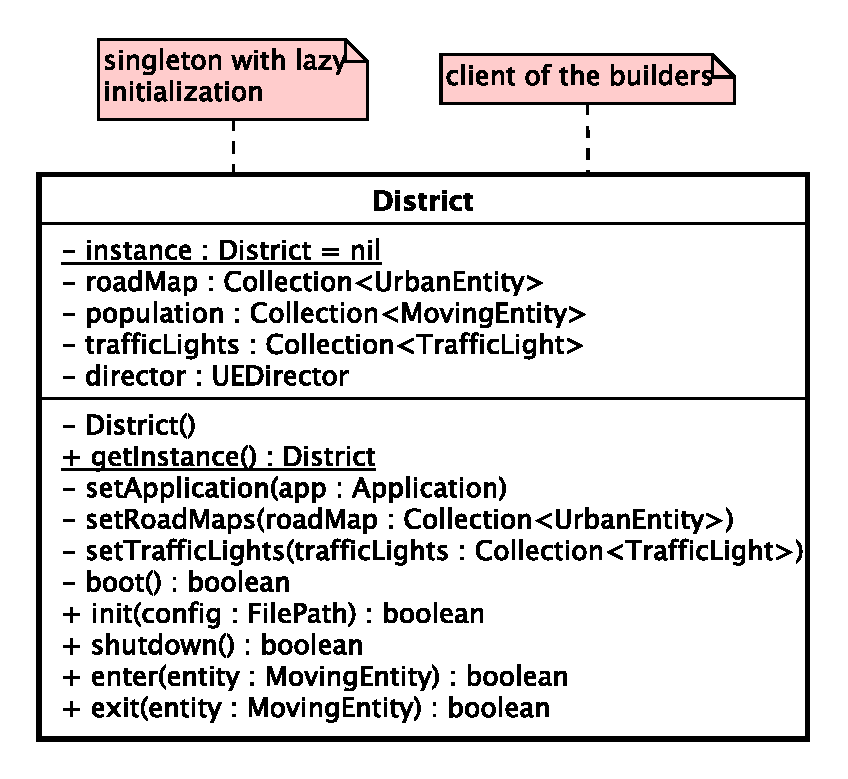
\includegraphics[scale=0.6,keepaspectratio]{images/solution/district.eps}
\caption{App::Reactive::District}
\label{fig:sd-app-district}
\end{figure}
\FloatBarrier
\begin{itemize}
  \item \textbf{Description} \\
It represents the master entity of the application layer. 
It has the responsibility to boot and shutdown the application layer.
  \item \textbf{Attribute}
  \begin{itemize}
    \item \texttt{- app: Application} \\
A reference to the interface of the application layer.
    \item \texttt{- roadMap: ArrayList<UrbanEntity>} \\
The urban entities of the district\footnote{Note that the name 
\textit{district} is only a convetion, indeed it is possible to have a 
real district splitted into different logical nodes of the system}
(i.e. crossroads and streets). 
    \item \texttt{- population: ArrayList<MovingEntity>} \\
The moving entities that reside on the district.
    \item \texttt{- trafficLight: ArrayList<TrafficLight>} \\
The traffic lights of the district.
    \item \texttt{- director: UEDirector} \\ 
The director of the city building process.
  \end{itemize}
  \item \textbf{Operation}
  \begin{itemize} 
    \item \texttt{- boot() : boolean} \\
Boots the application layer running all the active entities of the 
district (moving entities and traffic lights).
Returns true if the process completes neatly, false otherwise. 
This method is internally used by init.
    \item \texttt{+ init(config: FilePath) : boolean} \\
Creates and boots all the entities of the district according to the 
configuration file. Attaches each crossroads to the relative traffic light
if specified so in the configuration file. 
Returns true if the process completes neatly, false otherwise.
    \item \texttt{+ shutdown() : boolean} \\
Terminates the district. Returns true if the process completes neatly,
false otherwise.
    \item \texttt{+ enter(entity: MovingEntity) : boolean} \\
Notifies the district to add a new moving entity to the population.
Returns true if the process completes neatly, false otherwise.
    \item \texttt{+ exit(entity: MovingEntity) : boolean} \\
Notifies the district to pass a moving entity from the roadMap to the 
application layer interface which communicates to the middleware layer.
Returns true if the process completes neatly, false otherwise.
  \end{itemize}
\end{itemize} 
